Every learning algorithm is designed to learn concepts from a concept class $C$ but it does not know the target concept $c \in C$, and also the associated 
distribution $\boldsymbol{D}$. \vspace{7pt}

We would like anyway that our learning algorithm is able to learn from any possible distribution: for that main reason the distribution $\boldsymbol{D}$ of 
data cannot be known. \vspace{7pt}

The interface of any learning algorithm $A$ can be described as follows: \vspace{3.5pt}
\begin{center}
    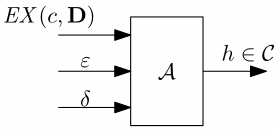
\includegraphics[width = 0.4\textwidth]{img/img11.png}
\end{center} \vspace{3.5pt}
where:
\begin{itemize}
    \renewcommand{\labelitemi}{-}
    \item $EX(c, \boldsymbol{D}) \rightarrow$ should be thought as an \textbf{oracle}, a procedure that $A$ can call as many times it wants, and which returns element $x \sim \boldsymbol{D}$ from the instance space $X$, labelled according to whether it is in the target class $c$ or not
    \item $\epsilon \rightarrow$ \textbf{error parameter}, it can be expressed also as the accuracy that we would like to achieve
    \item $\delta \rightarrow$ \textbf{confidence parameter}, the level of confidence should we achieve during the training
\end{itemize}
Therefore, the learning algorithm $A$ should be able to perform the oracle $EX(c, \boldsymbol{D})$ to get labelled data as many times it wants: during the 
training phase it should learn repetitive patterns from labelled data, giving us as final result a \textbf{hypothesis} $h \in C$. We would like a 
hypothesis $h$ that is as similar to the target class $c$ as possible. \vspace{7pt}

The \textbf{error} of any hypothesis $h \in C$ is defined as:
$$error_{\boldsymbol{D}, c}(h) = \text{Pr}_{x \sim \boldsymbol{D}}[h(x) \neq c(x)]$$
The \textbf{error} of a hypothesis $h$ with the respect to a target concept $c$ and a probability distribution $\boldsymbol{D}$ is defined as the probability that
$h$ and $c$ disagree on a randomly drawn point $x$.